\chapter{Background and Related Works}

%%%%%%%%%%%%%%%%%%%%%%%%%%%%%%%%%%%%%%%%%%%%%%%%%%%%%%%%%%%%%%%%%%%%%%%%%%%%%%%%%%%%%%%%%%%%%%%%%%%%

\section{ROS}

The \emph{Robot Operating System} (ROS) is an open-source framework for creating robot control systems, developed by \emph{Willow Garage} \cite{ros_paper}.

\subsection{Architecture}
ROS can be primarily thought of as a message-passing framework, similar to what is achieved by projects such as \emph{Erlang} \cite{erlang} and \emph{Akka}. A number of discrete processes, perhaps some even on a remote machine, communicate through a single broker service using an XMLRPC-based API. Each process performs a small part of a larger task, sharing data with other nodes through common data types, such that some robot control system can be implemented.

Each resource is given a name, and can be placed into a namespace. This gives each resource a unique \emph{graph resource name} which is the key method of referencing other parts of a system in ROS. As the name suggests, the layout of a ROS system can be thought of as a graph or tree. Some examples of \emph{graph resource names} are shown in Figure~\ref{fig:graph_resource_names}.

\begin{figure}[h!]
    \centering

    \texttt{/} (the global namespace)

    \texttt{/hexapod} (the \emph{hexapod} namespace)

    \texttt{/hexapod/servo\_controller} (a \emph{servo\_controller} node)

    \caption{An example of some graph resource names.}
    \label{fig:graph_resource_names}
\end{figure}

As touched on in the opening paragraph, ROS can function as a distributed system. Specifically, the processes can run on a machine different from that of the broker. The processes can then connect to the broker over some network. This can be used to offload complex computations onto another machine, should it be a requirement. To give an example, an embedded system running ROS on the robot can be collecting sensor data and issues hardware commands. This embedded system can then be communicating to a more powerful machine, acting as a base station. This base station can perform the more complex operations such as sensor data interpretation and path planning, relaying the commands back to the embedded system to be carried out.

\subsubsection{Processes as Nodes}
In ROS terminology, each of these processes are refereed to as a \emph{node}. A node is, simply, a process that is connected to the ROS broker, performing some sort computation \cite{ros_paper}.

One of the primary design concepts of ROS is that the framework should not be tied to any particular language \cite{ros_paper}. Nodes are developed using a ROS \emph{client library}, many of which are available. These are libraries in some form for a particular language or ecosystem, providing an abstraction for interfacing with ROS. The two key client libraries are \emph{roscpp} and \emph{rospy}, which are for C++ and Python respectively. There are a number of experimental client libraries for other systems, such as Java, Android, C\#, Arduino, and so on \cite{ros_wiki_clientlibraries}.

\subsubsection{Grouping Nodes in Packages}
A collection of nodes providing a particular set of functionalities (e.g., path planning for autonomous navigation), can be grouped and distributed as \emph{packages} \cite{ros_paper}. These packages can then be included into other projects, acting as a subsystem as part of a larger system.

Users of ROS are encouraged to share and distribute any developments they make by hosting repositories of their code, preferably on \emph{GitHub} \cite{ros_wiki_getinvolved}. Contributors can then request that their repository be listed on the ROS package index \cite{ros_wiki_getinvolved}. This aspect is a particularly key advantage of ROS, as there is a wide array of packages available. Additionally, as ROS provides a number of data types used in robotics, packages from different vendors can interact with one another with relative ease.

\subsubsection{Communicating Through Topics}
Nodes communicate with each other through \emph{topics} \cite{ros_paper}. On creation, a topic is given a particular \emph{message} type. Messages are simple data structures comprising of a number of typed data fields. Each data field has a unique name, and can be of a number of built-in primitive types, as well as other arbitrary data structures such as arrays and even other messages.

\subsubsection{Services}
ROS also provides a \emph{request-response} style method of communication through \emph{services} \cite{ros_wiki_services}.

\subsubsection{Parameters}
\emph{Parameters} provide a standard means for configuring ROS nodes and packages.

\subsection{Standard Packages \& Utilities}
\subsubsection{Launching Packages with roslaunch}
\subsubsection{Visualising Sensor Data with RViz}

%%%%%%%%%%%%%%%%%%%%%%%%%%%%%%%%%%%%%%%%%%%%%%%%%%%%%%%%%%%%%%%%%%%%%%%%%%%%%%%%%%%%%%%%%%%%%%%%%%%%

\section{Hardware}

The hardware involved in operating the robot used in this project is relatively straightforward. The robot is a hexapod, in that it has six limbs. Each limb has three joints at which it can rotate, as shown in Figure~\ref{fig:hexapod_dof}, giving three degrees-of-freedom per limb. 

\begin{figure}[!h]
    \centering
    (I am a diagram)
    \caption{This diagram shows the three degrees-of-freedom available to each limb on the robot.}
    \label{fig:hexapod_dof}
\end{figure}

In its current state, the robot has no wireless capability and, thusly, operates in a tethered manner. A bundle of cables protruding from the rear end of the unit connects the on-board hardware to a nearby power source and computer.

\subsection{Servos \& Servo Controller}
Each joint piece is attached to the shaft of a servomechanism (servo) to facilitate rotation. Each servo is controlled by a \emph{pulse-width modulated} (PWM) signal supplied by the controller, such that the angle of the servo can be controlled. Servos operate using a feedback-loop system such that the current of a motor is controlled, rotating the shaft to the desired position. Rotational range and speed of servos vary depending on model, but in this case the servos allow for a rotational range of 180 degrees.

\begin{figure}[!h]
    \centering
    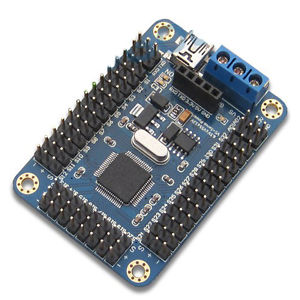
\includegraphics[width=6cm]{torobot_controller}
    \caption{The \emph{Torobot 32-Channel Servo Controller}, as used in the hexapod.}
    \label{fig:torobot_controller}
\end{figure}

The servos are controlled by an off-the-shelf servo controller board. This board, in particular, expects text-based control commands over serial, either via direct TTL or emulated over an on-board USB to TTL converter \cite{torobot_manual}. A number of commands are supported, allowing control of the position of both single and groups of servos. Additionally, a set of movements can be programmed and issues with a single command \cite{torobot_manual}. Power is also distrusted to the servos via this board.

The servo controller itself is powered by a standard laboratory power supply.

\subsubsection{Protocol}

Commands are issues via a simple ASCII-based protocol, over serial communication. The controller expects serial communication to operate with the following parameters \cite{torobot_manual}.

\begin{itemize}
    \item 9600bps baud rate.
    \item No check bits.
    \item 8 data bits.
    \item 1 stop bit.
\end{itemize}

While the servo controller supports a number of commands, we use only the command which rotates an individual servo. This allows us to be more flexible in terms of when movement begins, as all servos mentioned in a group command will begin moving at the same time.

\begin{figure}[!h]
    \centering
    \texttt{\#\(n\)\#P\(a\)T\(t\)\emph{\textbackslash r\textbackslash n}}
\end{figure}

A rotation command is issued by sending a string in the format shown above, specifying the particular servo number (\(n\)), the target angle (\(a\)), and the time over which the rotation should occur (\(t)\) in milliseconds. In particular, it should be noted that the parameter for the target angle is actually the pulse width duration that is sent to the servo.

\subsection{RGB-D Sensor}
The primary sensor in the system is an \emph{ASUS Xtion Pro Live} RGB-D sensor, which is very similar to the \emph{Microsoft Kinect}. The key functionality of this sensor is that it provides a depth video feed, giving a range of values indicating the distances to the objects in front of it.

Whole bunch of example pictures of how it works, what it does, etc.

The advantages this particular sensor provides over the \emph{Kinect} is mostly physical, specifically weight and footprint. The \emph{Kinect} has a motorized base which allows the device to be tilted upwards and downwards through software, in comparison to the \emph{Xtion} which has a simple hinge that can be rotated by hand. This feature is unnecessary in this use case and adds a significant amount of weight. Additionally, the \emph{Kinect} is intended to be a consumer device and, thus, has a much striking product design. However, this striking design comes at a cost of making the device much larger in general, which is somewhat troubling when it must be placed on an already space-starved robot base.

%%%%%%%%%%%%%%%%%%%%%%%%%%%%%%%%%%%%%%%%%%%%%%%%%%%%%%%%%%%%%%%%%%%%%%%%%%%%%%%%%%%%%%%%%%%%%%%%%%%%

\section{Existing Examples}